\subsection{Experiment}
\label{subsec:toro_exp}
The estimation problem is tested in Matlab Simulink. The experimental setup consists of the Open HRP3 simulator and the state estimator. The OpenHRP3 (Open Architecture Human-centred Robotics Platform version 3) is an integrated software platform for robot simulations and software developments \footnote{\url{http://www.openrtp.jp/openhrp3/en/about.html}}. It was developed as a cooperative work of University of Tokyo, General Robotix. Inc and National Institute of Advanced Industrial Science and Technology(AIST).

\begin{figure}[H]
    \centering
    % We need layers to draw the block diagram
\pgfdeclarelayer{background}
\pgfdeclarelayer{foreground}
\pgfsetlayers{background,main,foreground}

% Define a few styles and constants
\tikzstyle{sensor}=[draw, fill=blue!20, text width=5em,text centered, minimum height=2.5em]
\tikzstyle{system} = [sensor, text width=6em, fill=green!30, 
    minimum height=12em, rounded corners]
\tikzstyle{input} = [coordinate]
\tikzstyle{sum} = [draw, fill=blue!20, circle, node distance=1cm]
%\tikzstyle{output} = [coordinate]
\def\blockdist{0.5}
\def\edgedist{0.75}
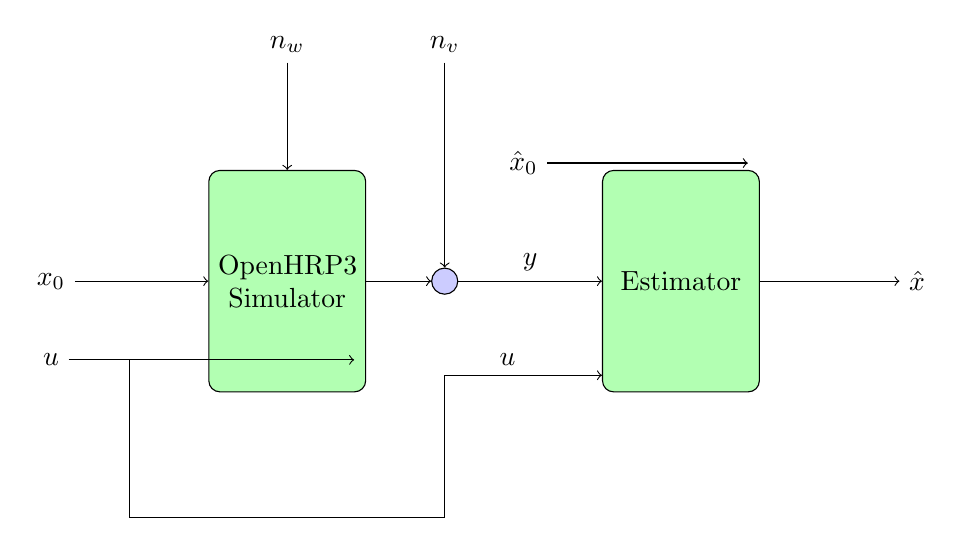
\begin{tikzpicture}
	% Define the nodes in the picture
	\node (sys_in)[yshift=1cm]{$x_0$};
	\node (u_in) [below of=sys_in,node distance=1cm]{$u$};
	\node (sys_u)[input,right of=u_in,node distance=1cm]{};
    \node (sim_sys) [system,right of=sys_in,node distance=3cm] {OpenHRP3 Simulator};
    \node (sys_noise)[above of=sim_sys,node distance=3cm]{$n_w$};
    \node (msr_noise)[right of=sys_noise,node distance=2cm]{$n_v$};
    \node (msr_add)[sum,right of=sim_sys,node distance=2cm]{};
    \node (estimator) [system,right of=msr_add,node distance =3cm]{ Estimator};
    \node (est_in) [right of=sim_sys,node distance=3cm,yshift=1.5cm]{$\hat{x}_0$};
    \node (est_u) [input,right of =sim_sys, node distance=2cm,yshift=-3cm]{foo};
    \node (est_out)[right of=estimator,node distance=3cm]{$\hat{x}$};
    
    % Define the edges in the picture
    \draw [->] (sys_in) --node{}(sim_sys.west);
    \draw [-] (u_in) --node{}(sys_u);
    \draw [->] (sys_u) --node{}+(\edgedist,0);
    \draw [-] (sys_u) |-node{}(est_u);
    \draw [->] (est_u) |-node[pos=0.7,above]{$u$}(estimator.-130);
    \draw [->] (est_in) --node{}+(\edgedist,0);
    \draw [->] (sys_noise) --node{}(sim_sys.north);
    \draw [->] (msr_noise) --node{}(msr_add.north);
    \draw [->] (sim_sys.east) --node[above]{}(msr_add.west);
    \draw [->] (msr_add.east) --node[above]{$y$}(estimator.west);
    \draw [->] (estimator) --node{}(est_out);
\end{tikzpicture}
    \caption{Experimental setup of TORO}
    \label{fig:toro_exp}
\end{figure}

A rigid body algorithm is used in the estimator to compute dynamic $M(y_k), C(y_k,\dot y_k), g(y_k)$ and kinematic $J_r(y_k), J_l(y_k), H(y_k)$ parameters at time step $k$. An auto differentiation function that computes the derivative of the dynamic and kinematic parameters with respect to the the system states is integrated with the rigid body algorithm. 
\begin{figure}[H]
    \centering
    % We need layers to draw the block diagram
\pgfdeclarelayer{background}
\pgfdeclarelayer{foreground}
\pgfsetlayers{background,main,foreground}

% Define a few styles and constants
\tikzstyle{sensor}=[draw, fill=blue!20, text width=5em,text centered, minimum height=2.5em, rounded corners]
\tikzstyle{system} = [sensor, text width=5em, fill=green!30, 
    minimum height=8em]
%\tikzstyle{input} = [coordinate]
\tikzstyle{sum} = [draw, fill=blue!20, circle, node distance=1cm]
\tikzstyle{output} = [coordinate]
%\def\blockdist{0.5}
\def\edgedist{2.85}
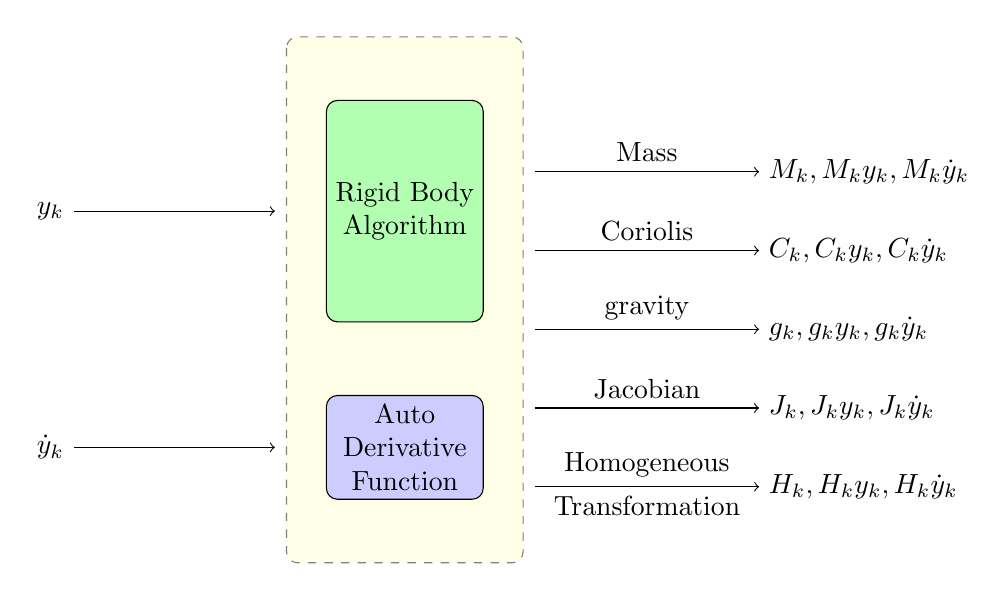
\begin{tikzpicture}
	% Define the nodes in the picture
	\node (y)[yshift=1cm]{$y_k$};
	\node (dy) [below of=y,node distance=3cm]{$\dot y_k$};
    \node (rigbdy_alg) [system,right of=y,node distance=4.5cm] {Rigid Body Algorithm};
    \node (auto_diff) [ sensor,below of=rigbdy_alg,node distance =3cm]{Auto Derivative Function};
    \node (M) [output,right of=rigbdy_alg,node distance=1.65cm,yshift=0.5cm]{};
    \node (C) [output,below of=M,node distance=1cm]{};
    \node (g) [output,below of=C,node distance=1cm]{};
    \node (J) [output,below of=g,node distance=1cm]{};
    \node (H) [output,below of=J,node distance=1cm]{};

    % Define the edges in the picture
    \draw [->] (y) --node{}+(\edgedist,0);
    \draw [->] (dy) --node{}+(\edgedist,0);
    \draw [->]  (M) --node[above]{Mass}+(\edgedist,0) node[right]{$M_k, \dfdx{M_k}{y_k},\dfdx{M_k}{\dot y_k}$};
    \draw [->]  (C) --node[above]{Coriolis}+(\edgedist,0) node[right]{$C_k, \dfdx{C_k}{y_k},\dfdx{C_k}{\dot y_k}$};
    \draw [->]  (g) --node[above]{gravity}+(\edgedist,0) node[right]{$g_k, \dfdx{g_k}{y_k},\dfdx{g_k}{\dot y_k}$};
    \draw [->]  (J) --node[above]{Jacobian}+(\edgedist,0) node[right]{$J_k, \dfdx{J_k}{y_k},\dfdx{J_k}{\dot y_k}$};
    \draw [->]  (H) --node[above]{Homogeneous} node[below]{Transformation}+(\edgedist,0) node[right]{$H_k, \dfdx{H_k}{y_k}, \dfdx{H_k}{\dot y_k}$};
    
    %Draw background layers
    \begin{pgfonlayer}{background}
        % Compute a few helper coordinates
        \path (auto_diff.west |- rigbdy_alg.north)+(-0.5,0.8) node (a) {};
        \path (auto_diff.south -| rigbdy_alg.east)+(+0.5,-0.8) node (b) {};
        \path[fill=yellow!10,rounded corners, draw=black!50, dashed]
            (a) rectangle (b);
    \end{pgfonlayer}
%\end{comment}
\end{tikzpicture}

    \caption{Structure of rigid body algorithm}
    \label{fig:luc_dyn}
\end{figure}
The Jacobian $J_k$ outputted by the algorithm shown in Figure \ref{fig:luc_dyn} is the body Jacobian of \emph{Toro's} right foot $J_r$ and left foot $J_l$ and homogeneous transformation matrix $H_k$ is the transformations of right foot $H_r$, left foot $H_l$ and floating base $H_b$ with respect to spatial frame (world frame).
The Jacobian matrices $A_k$ and $\hat C_{k+1}$ in Equations \ref{eq:sys_mat}, \ref{eq:msr_mat} are computed from these outputs of the rigid body algorithm. The formulation of the Jacobian matrices $A_k$ and $\hat C_{k+1}$ are discussed in sections \ref{subsec:toro_predict} and \ref{subsec:toro_update}. 

The simulator is driven by the control input $u$. For instance the control input of \emph{Toro} are the torque applied to joints $\tau$. The controller generates these inputs according to the control law. These inputs can be measured with the help of the torque sensors located at the joints. The ground reaction forces $W_r$ and $W_l$ are measured by the Force Torque sensor (FTS) located at the ankle joints. The ground reaction forces and the control torques are the input to prediction model in Equation \ref{eq:toro_dis}.

The following scenario is simulated using the OpenHRP3 simulator. It consists of the following phases:

\paragraph{Initial phase:} The robot is made to stand on the ground (high pose). After a few seconds the robot is commanded to move to a different pose (medium pose) by applying the control inputs $u$. 

\begin{figure}
	\centering
	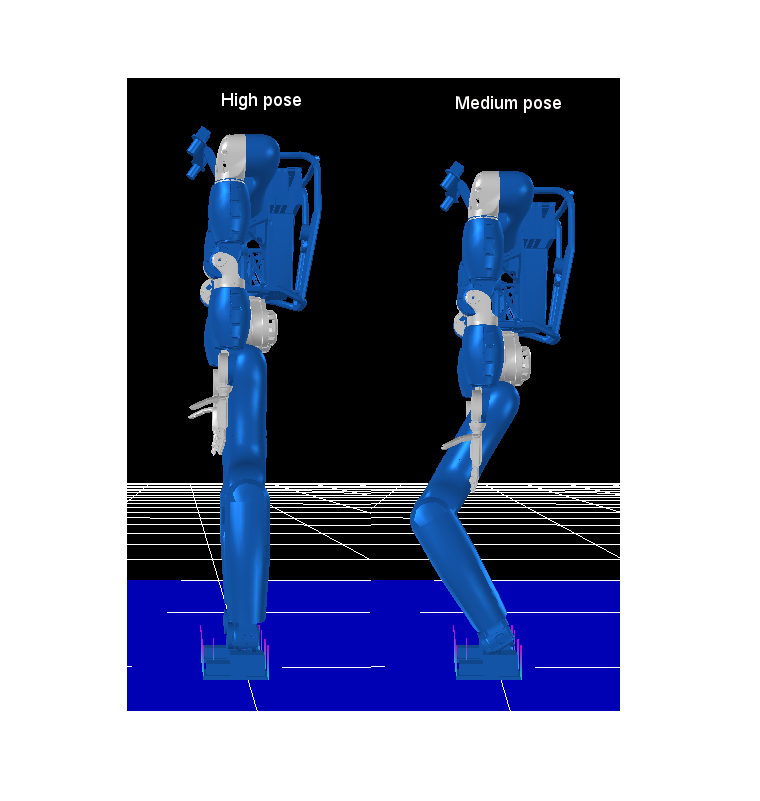
\includegraphics[width=0.7\textwidth,height=0.4\textheight]{Bilder/toro_high_medium.png}
	\caption{Snapshots of two different pose of \emph{Toro} in OpenHRP3 simulation}
	\label{fig:toro_sim_high_low}
\end{figure}
\begin{figure}
	\centering
	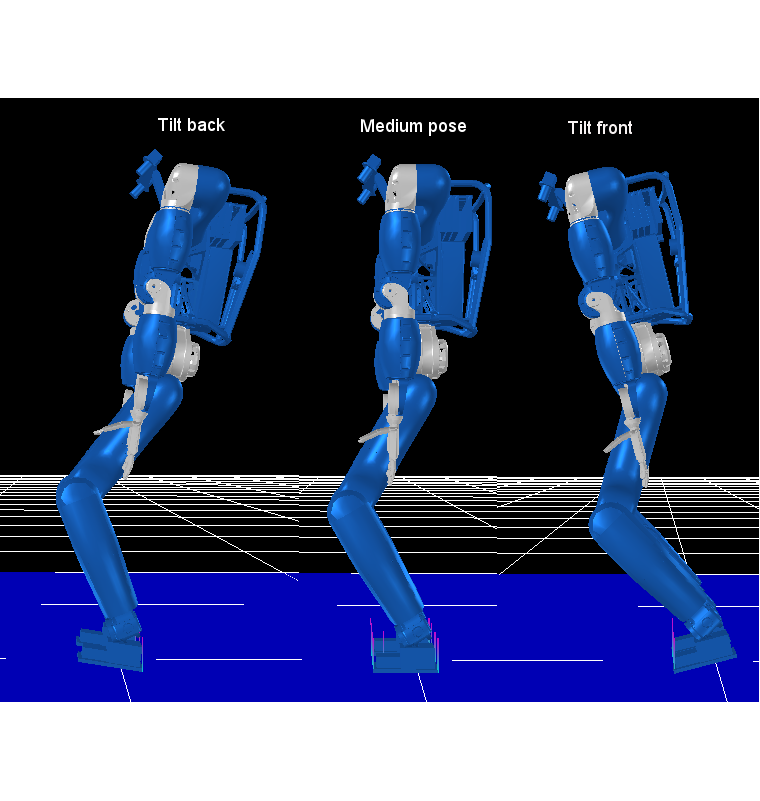
\includegraphics[width=0.7\textwidth, height=0.4\textheight]{Bilder/toro_tiltphase.png}
	\caption{Snapshots of tilting phase of \emph{Toro} in simulation}
	\label{fig:toro_tiltphase}
\end{figure}

\paragraph{Tilting phase:} After a few seconds an external force is applied to the robot so that it starts to tilt around an edge. After the robot has tilted few degrees the external force is removed,as a result the robot goes back to the medium pose due to inertia of the upper body. The robot stores the energy when the force is applied, it is not completely dissipated when it comes back to the medium pose. Inorder to dissipate the stored energy, it tilts in the other direction and then move back due to inertia. This cycle goes on until the robot dissipates all its stored energy. After the energy is dissipated the robot stays in the medium pose.
\paragraph{Final phase:} After the tilting phase is complete the robot is commanded to move back to the high pose.

The simulations and estimation are made with an integration time step of $\Delta t=1ms$. Zero mean Gaussian noises $w$ and $v$ are added to the inputs and measurements.
\begin{table}[H]
    \centering
    \begin{tabular}{|c|c|}
    \hline
    Name of the sensor &Noise variance \\ \hline
    \textbf{Input noise} &\hspace{2mm}\\
    FTS $W_r,W_l$ & $1 \cdot {10}^{-2}$ \\ 
    Torques $\tau$ & $1 \cdot {10}^{-4}$\\    \hline
    \textbf{Measurement noise} &\hspace{2mm}\\
    Joint angles $q(rad)$ &$1\cdot{10}^{-6}$ \\ 
    Joint velocities $\dot q(rad/s)$ &$1\cdot{10}^{-4}$ \\
    Acceleration $\dot v^b(m/s^2)$ &$1\cdot{10}^{-2}$ \\ 
    Angular velocity $\omega^b(rad/s)$ &$1\cdot{10}^{-4}$ \\ \hline
    \end{tabular}
    \caption{Variance of simulated noises}
    \label{tab:toro_var}
\end{table}

The values of the process and measuremt covariance matrices $Q$ and $R$ are set with the variance of the noises from Table \ref{tab:toro_var}. They are 
$$  \begin{aligned}
         Q &= diag([1\cdot{10}^{-2} \textbf{1}_{12,1}; 1\cdot{10}^{-4} \textbf{1}_{25,1}])  \\
         R &= diag([1\cdot{10}^{-6} \textbf{1}_{25,1}; 1\cdot{10}^{-4}\textbf{1}_{25,1}; 1\cdot{10}^{-2}\textbf{1}_{3,1};1\cdot{10}^{-4}\textbf{1}_{3,1}; 1\cdot{10}^{-12}\textbf{1}_{36,1} ]),
     \end{aligned}$$
where $\textbf{1}_{r,c}$ is the matrix of dimensions $r \times c$ with all the elements as 1 [Appendix \ref{sec:symbols}] and $diag(x)$ is a diagonal matrix where the main diagonal entries are the elements of vector $x$. 
The initial values of the system $x_0$ and estimator $\hat x_0$ are
$$ \begin{aligned} x_0 &= [0,0,1.164,\textbf{0}_{1,59}]^T \\ \hat x_0 &= \textbf{0}_{62,1}, \end{aligned} $$  where $\textbf{0}_{62,1}$ is the zero matrix of dimensions $62 \times 1$ [Appendix \ref{sec:symbols}].
The initial value of the covariance matrix $P_0$ is $$ P_0 = I_{62},$$ where $I_{62}$ respresents the identity matrix of dimensions $62\times62$. 

\subsubsection{Observation}
\begin{figure}
    \centering
%    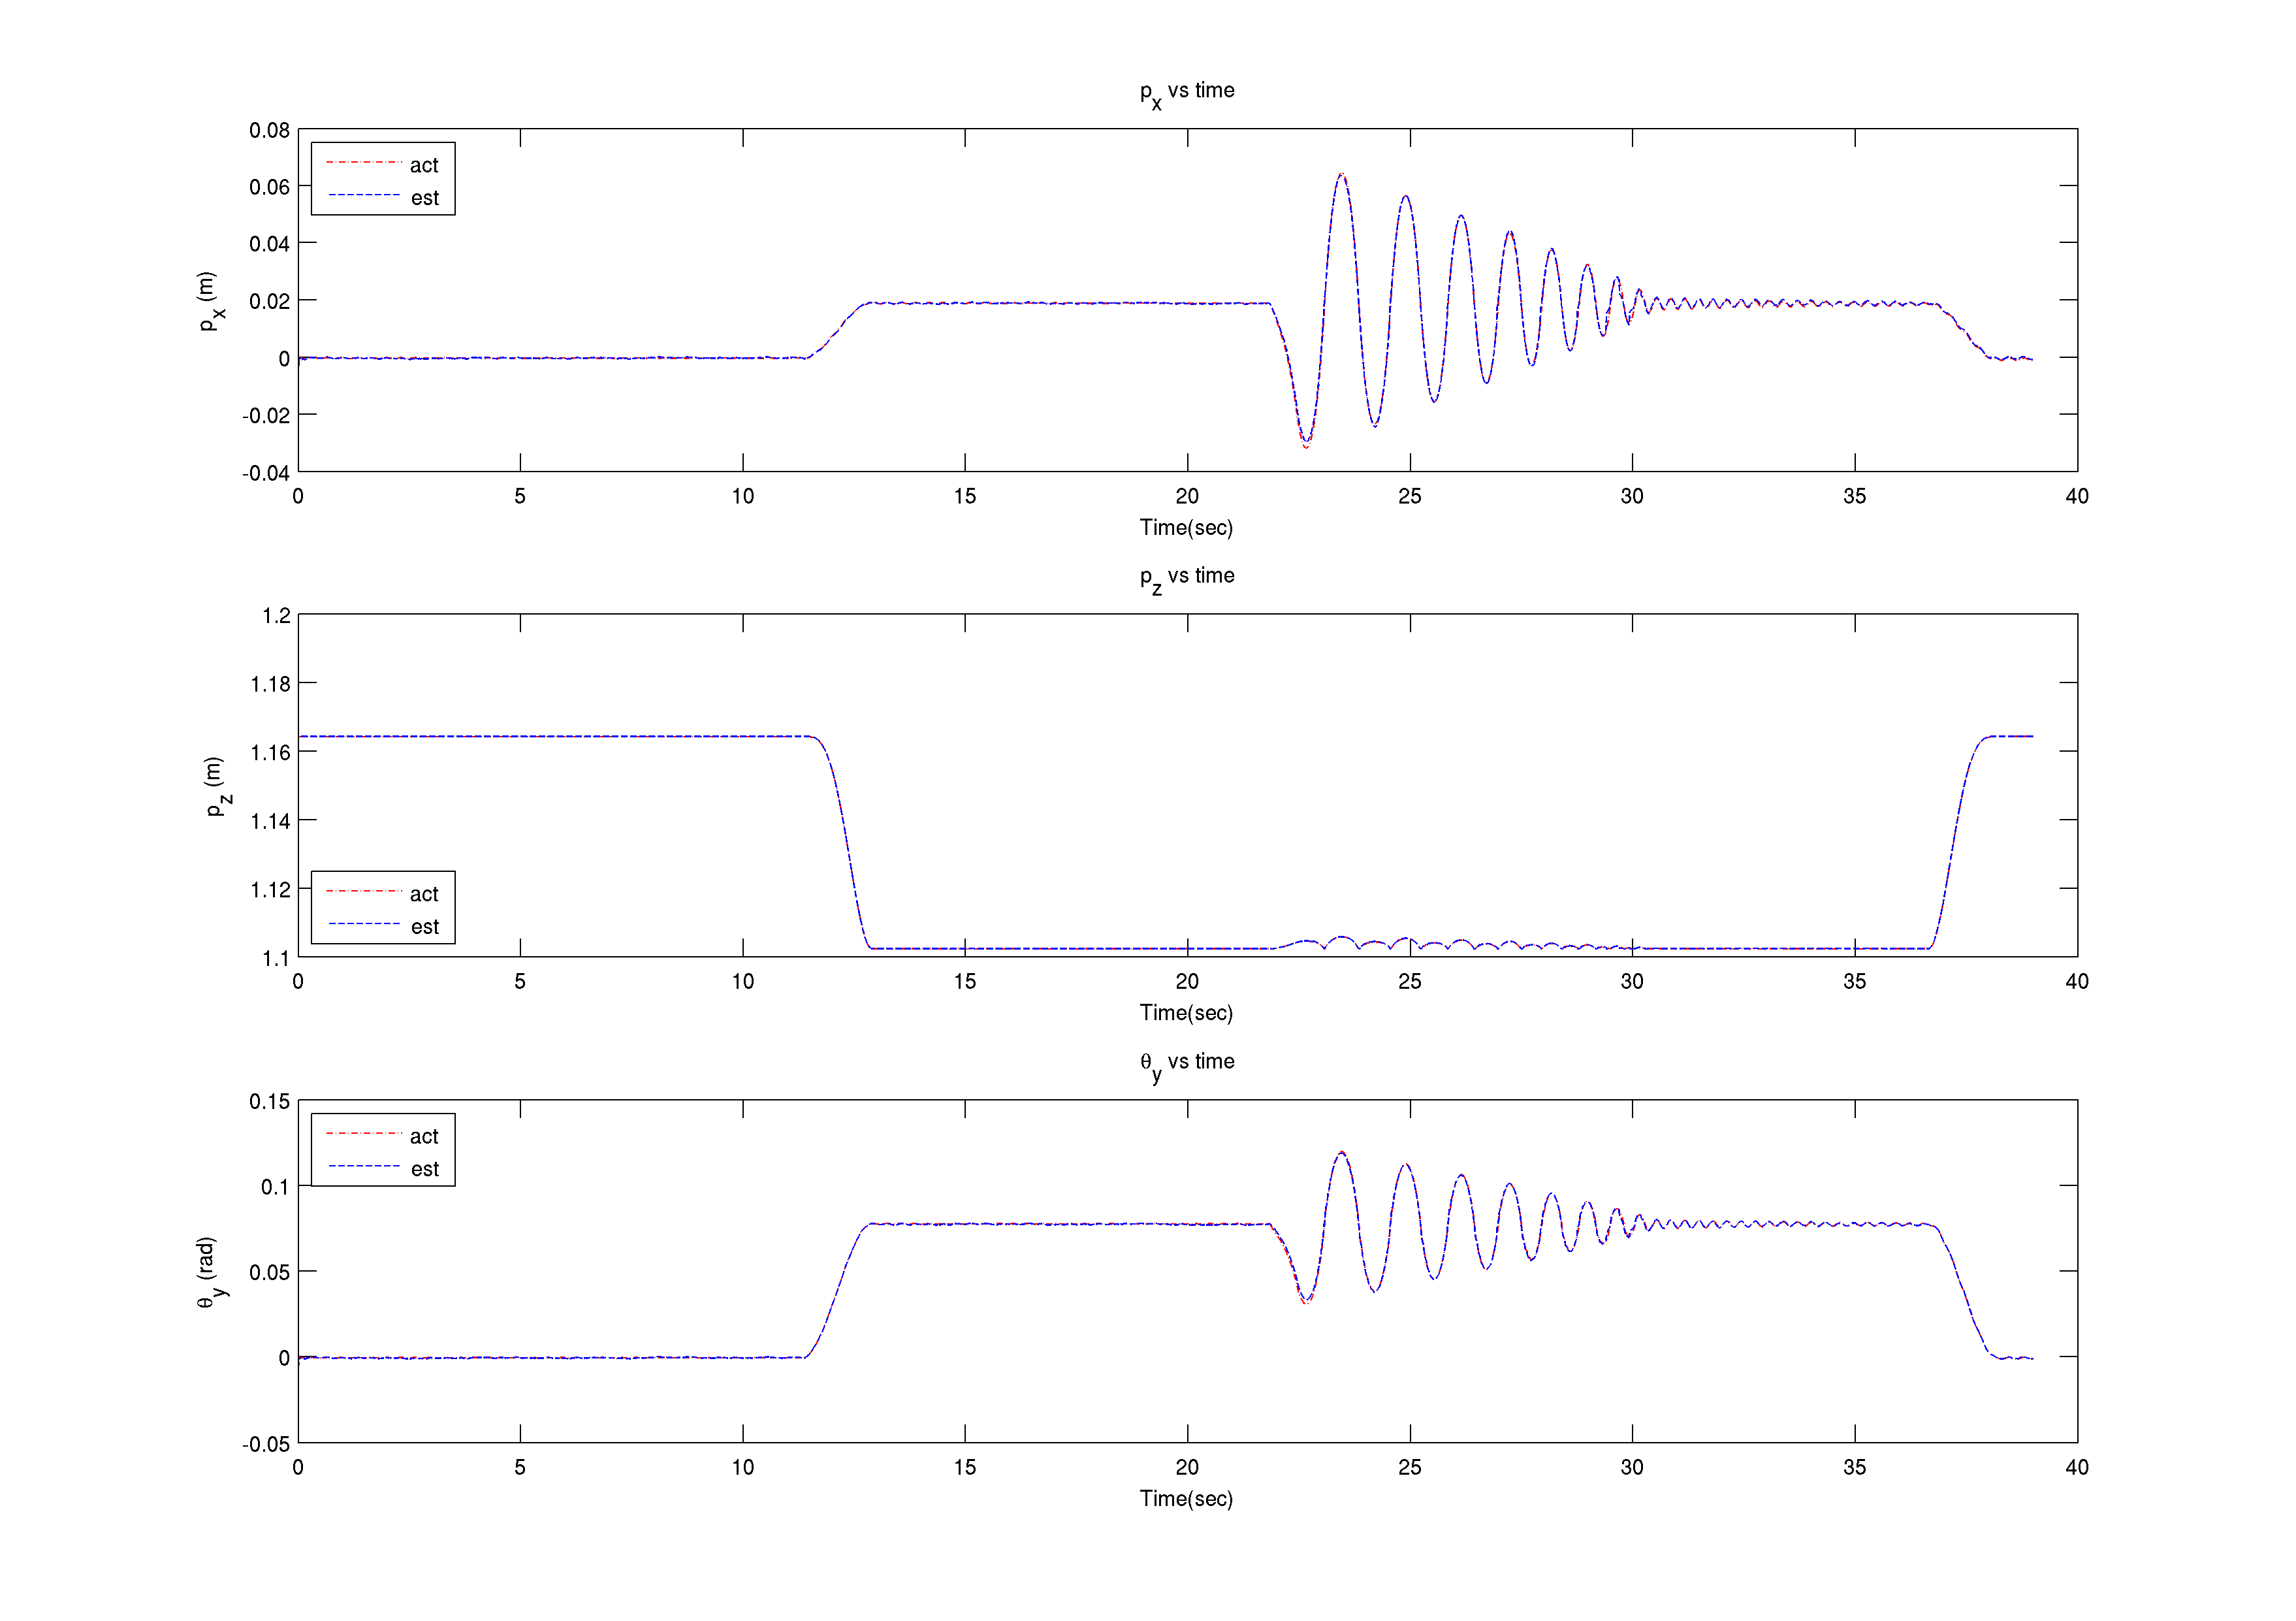
\includegraphics[height=0.5\textheight width=0.8\textwidth]{Bilder/plots/toro/toro_pos.png}
    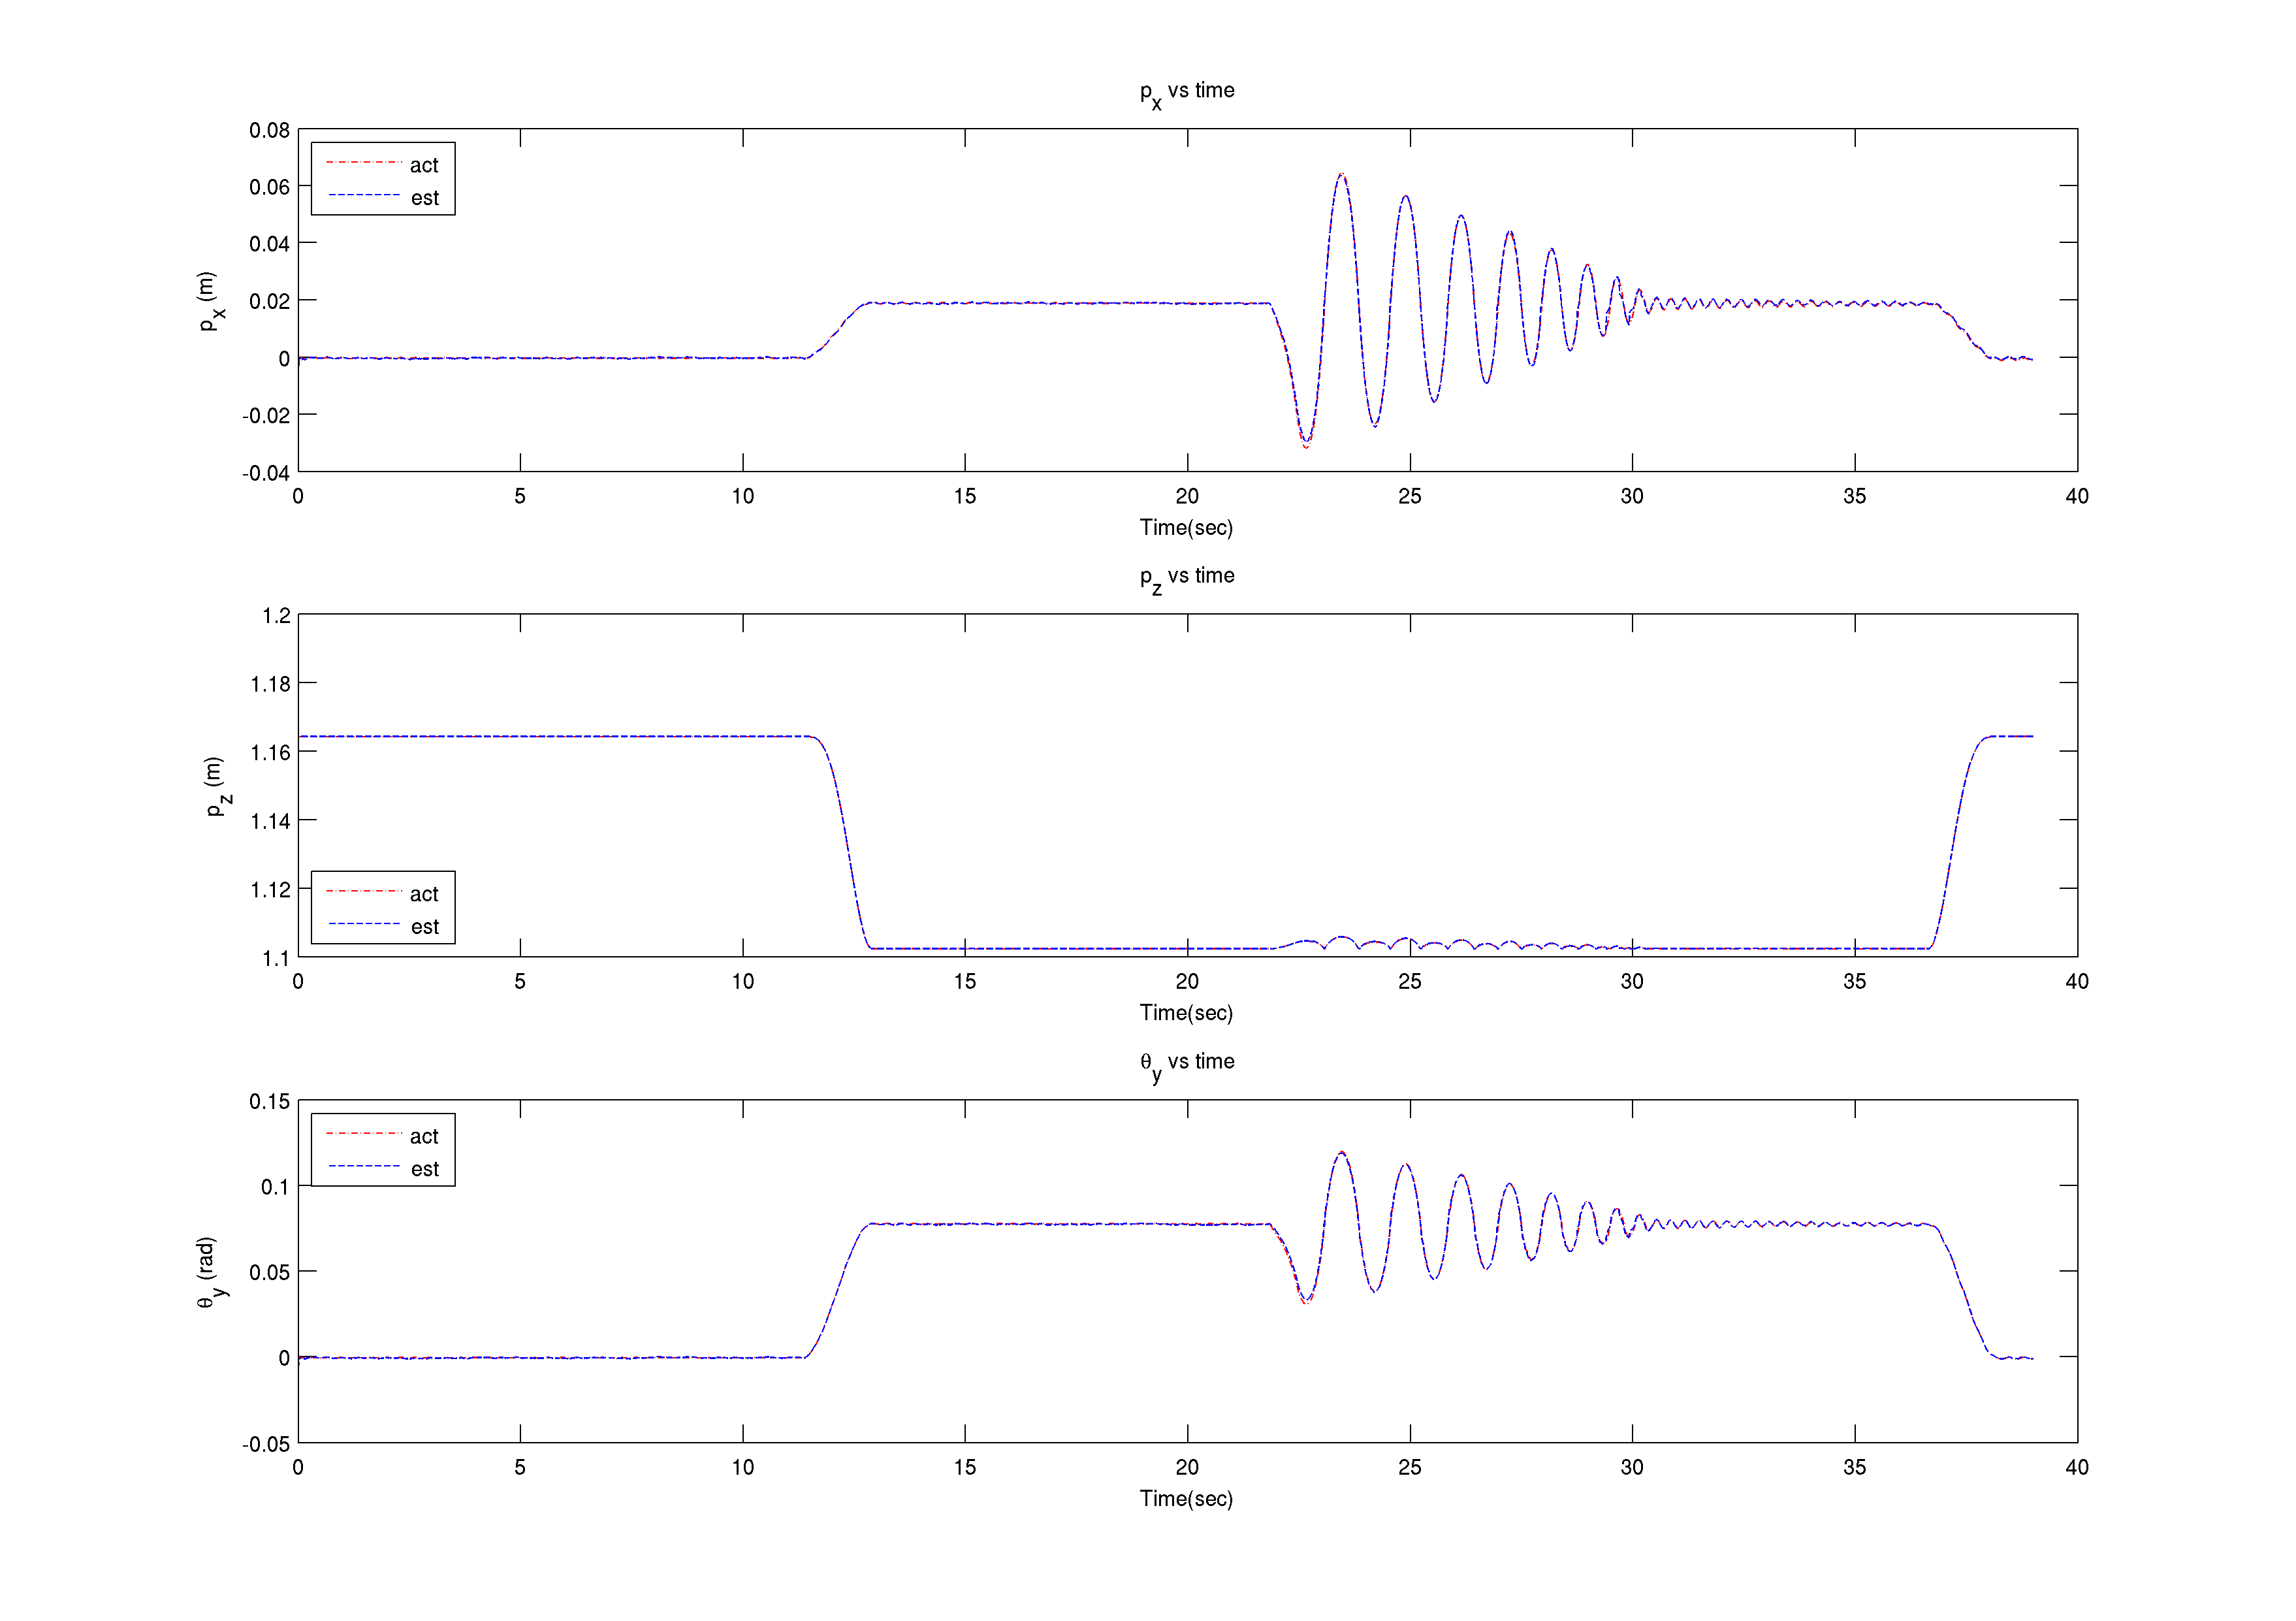
\includegraphics[trim=25mm 10mm 25mm 10mm,clip,scale=0.6]{Bilder/plots/toro/toro_pos.png}
    \caption{Actual and estimated values of $p_x,p_z$ and $\theta_y$}
    \label{fig:toro_plotpos}
\end{figure}
\begin{figure}
    \centering
    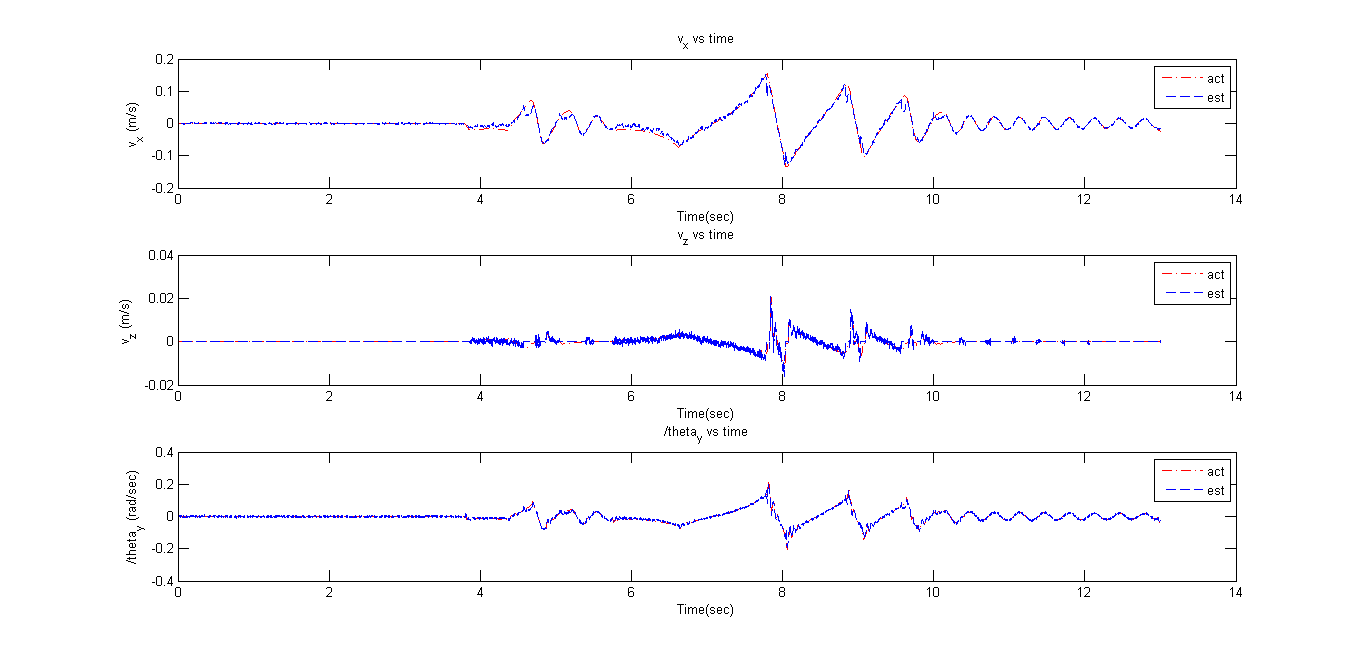
\includegraphics[trim=25mm 10mm 25mm 10mm,clip,scale=0.55]{Bilder/plots/toro/toro_vel.png}
    \caption{Actual and estimated values of $v_x,v_z$ and $\omega_y$}
    \label{fig:toro_plotvel}
\end{figure}

The robot tilts about the front and back edges of the foot. In other words it rotates about the $Y-axis$ of the spatial frame (world frame). A rotation of $\theta_y$ around $Y-axis$ will results in translation motions $p_x$ and $p_z$ along $X$ and $z$ axes. These three quantities are plotted in Figure \ref{fig:toro_plotpos}. The velocities of these quantities $\omega_y,v_x,v_z$ are plotted in Figure \ref{fig:toro_plotvel}.

In the the Figures \ref{fig:toro_plotpos} and \ref{fig:toro_plotvel} the time interval between $0-22s$ denotes the \emph{initial phase}, $22s-35s$ denotes the \emph{tilting phase} and $35s-39s$ denotes the \emph{final phase}. We can see in the above figures that, the estimates converges quickly to the actual states. 
\begin{table}[H]
    \centering
    \begin{tabular}{|c|c|}
    \hline
    Estimates &RMSE \\ \hline
    $\hat p_x$ &0.0005 $m$\\
    $\hat p_y$ &0.0001 $m$\\
    $\hat p_z$ &0.0001 $m$\\
    $\hat\theta_x$ &0.0001 $rad$\\
    $\hat\theta_y$ &0.0006 $rad$\\
    $\hat\theta_z$ &0.0001 $rad$\\ \hline
    \end{tabular} \hspace{1cm}
    \begin{tabular}{|c|c|}
    \hline
    Estimates &RMSE \\ \hline
    $\hat v_x$ &0.0083 $m/s$\\
    $\hat v_y$ &0.0017 $m/s$\\
    $\hat v_z$ &0.0040 $m/s$\\
    $\hat\omega_x$ &0.0013 $rad/s$\\
    $\hat\omega_y$ &0.0042 $rad/s$\\
    $\hat\omega_z$ &0.0060 $rad/s$\\ \hline
    \end{tabular}
    \caption{RMSE values of the position and velocity estimates of the floating base}
    \label{tab:toro_rmse}
\end{table}

The RMSE values of the estimates in Table \ref{tab:toro_rmse} are small. This shows that EKF has a good performance for the given prediction system model. The joint angles $ \hat q \in \Re^{25}$ and velocities $\hat \dot q \in \Re^{25}$ are also well estimated by the EKF. Since we focus on estimating the motion parameters of floating base, the joint's motion parameters are not discussed.

The time taken for 10 seconds of simulation of the EKF is $1290$ seconds. For each integration time step ($\Delta t = 0.001 s$) the EKF requires $0.129 s$ in real time for its execution. The high computation time is caused by the rigid body algorithm which has an execution time of $0.06s$. This algorithm is executed two times per time step.
$$ \text{Time take for the execution of rigid body algorithm } = 2 \times 0.06 = 0.12 s.$$ This is approximately the execution time of the EKF for one time step.

\subsection{Conclusion}
The state estimation of motion parameters of under-actuated degrees of freedom is the main aim in this thesis. With the multibody dynamic model of \emph{Toro} it is possible to estimate more than the under-actuated degrees of freedom. 
